\documentclass[a4paper,12pt]{article}

\usepackage[french]{babel}
\usepackage[utf8]{inputenc}
\usepackage{graphicx}


\title{Cahier des charges du ProjetNigma}
\author{CrypTeam}
\pagestyle{myheadings}
\date{}

\begin{document}
	\markright{Cahier des charges de la CrypTeam}
	\maketitle{}
  	\tableofcontents
	\newpage
	\part{Introduction}
	%introduction rapide
        \section {Présentation de la CrypTeam}
        \section {Présentation individuelle}
        \subsection{Guillaume LAPOTRE}
        \subsection{Justin GANIVET}
        \subsection{Stéphane LADEVIE}
        \subsection{Sébastien GISLAIS}
	\newpage
	\part{\'{E}tat de l'art}
		La cryptographie et la stéganographie sont deux techniques extrêmement ancienne permettant de transmettre des informations uniquement aux personnes voulues.

 La cryptographie protège le message en le chiffrant, c'est-à-dire en le rendant incompréhensible sans connaitre l'algorithme de cryptage. On peut citer comme procédé de cryptage historique le chiffre de César qui décale l'alphabet de n rang suivant le chiffre choisi (ainsi si le chiffre choisi est 3, l'alphabet sera : DEFGHI...ZABC).

	La stéganographie consiste à cacher le message à transmettre plutot que de le chiffrer. Comme exemple historique on peut citer un procédé utilisé par César, il écrivait sur le crane d'un esclave un message puis attendait que les cheveux de cet esclave repoussent puis il envoyait l'esclave à la personne à qui le message était destiné. Il suffisait donc de raser l'esclave pour récupérer le message.

	Cepandant, la stéganographie ainsi que la cryptographie étaient utilisée quasiment uniquement par les militaires avant la fin de la Seconde Guerre Mondiale. Depuis, il y a énormément d'application civile au chiffrement
		\section{Cryptographie}
			\subsection{Cryptage par substitution}
	Le cryptage par substitution  est une des technique les plus basique et les plus ancienne de chiffrement. Le chiffre de César est une technique de cryptage par substitution. Il existe plusieurs types de substitution pour chiffrer des données.

	\subsubsection{Le cryptage par substitution mono-alphabétique}
	On remplace chaque lettres de l'alphabet par une autre lettre. Ainsi pour la première lettre il y a 26 possibilités, pour la seconde 25 possibilités etc\dots Il existe donc 26! façons de coder distinctes. L'inconvénient de la substitution mono-alphabétique est qu'il faut se souvenir de chaque substitutions pour chaques lettres. L'autre inconvénient est qu'en connaissant la langue du message codé on peut relativement facilement déchiffrer le message en se basant sur la fréquence d'apparition de chaque lettre dans une langue. Par exemple en français la lettre apparaissant le plus souvent est le E, en analysant un texte chiffré avec cette technique de chiffrement, on peut trouver la lettre qui apparait la plus souvent et l'associer donc à la lettre E. Ensuite on utilise le même raisonnement pour toute les autres lettres.

	\subsubsection{Le codage par substitution poly-alphabétique}
	Le chiffre de Vigenère en est un exemple. On crée un mot qui sert de clé et "on le colle en dessous du texte à chiffrer". Pour chiffrer ou déchiffrer un message on utilise une matrice 26x26 avec l'alphabet sur la première ligne et sur la première colonne. Ensuite on chiffre chaque lettre à l'aide de la lettre de la clé que l'on a disposé juste en dessous avec la matrice ci-dessous.
\begin{center}
	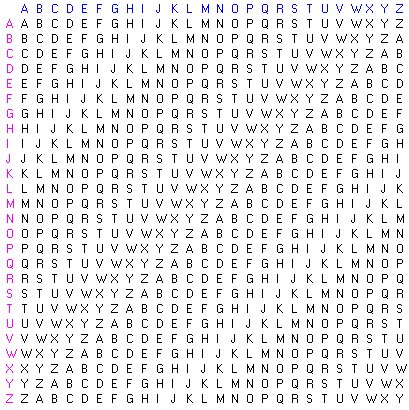
\includegraphics[scale=0.75]{../Image/matrice.jpg}
\end{center}
	Exemple : Chiffrons le mot Poney à l'aide de la clé EPITA : \\ P o n e y \\E P I T A \\
	Poney chiffré avec cette clé :
\begin{itemize}
\item P crypté avec la lettre E : T
\item O crypté avec la lettre P : D
\item N crypté avec la lettre I : V
\item E crypté avec la lettre T : X
\item Y crypté avec la lettre A : Y
\end{itemize}
	Poney crypté à l'aide de la clé EPITA avec le chiffre de Vigenère donne TDVXY !

			\subsection{Cryptage symétrique}
			\subsubsection{DES}
			\subsubsection{AES}

			\subsection{Cryptage asymétrique}
			\subsubsection{RSA}
 Le RSA est un algorithme méthode de cryptographie inventée en 1977 par  Ron Rivest, Adi Shamir, Len Adleman (d'où le nom de RSA). C'est encore le système cryptographique à clé publique le plus utilisé de nos jours.

Petite anecdote : Au départ, Rivest, Shamir et Adleman voulaient prouver que tout système à clé plublique possède une faille, c'est ainsi qu'ils ont créé le RSA !

 Son principe de fonctionnement suit 4 étapes : \\
 Tout d'abord il y a la création des clés(que l'on nommera p,q,e et d). P et Q sont deux grands nombres premiers distincts. Leur génération se fait au hasard en utilisant un algorithme de test de primalité probabiliste. C'est un algorithme qui determine si un nombre est probablement premier selon le degré de probabilité que l'on a fixé dans l'algorithme. En cryptographie, on se "contente" d'avoir un nombre dont on sait qu'il est premier avec une probabilité supérieur à \begin{math} 1- \frac{1}{2^{100}} \end{math}. E est un entier premier avec le produit (P-1)(Q-1). D est tel que ED = 1 mod (P-1)(Q-1) donc que ED -1 est un multiple de(P-1)(Q-1). On peut fabriquer D à partir de E, P et Q en utilisant l'algorithme d'Euclide.

Ensuite il faut distribuer les clés. Le couple (n,e) constitue la clé publique. Elle est disponible pour toute personne voulant crypter un message afin de nous l'envoyer ensuite. Le couple (n,d) constitue notre clé privée que l'on garde secrète. Si une personne désire nous envoyer un message codé, elle le représente sous la forme de plusieurs entiers M compris entre 0 et n-1. Elle possède notre clé publique (n,e) et calcule \begin{math}C = M^{e} \ mod\ n\end{math}. C'est ce dernier nombre qu'elle nous envoie.

Nous recevons donc C et on calcule grace à notre clé privée \begin{math}D = C^{d}\ mod\ n\end{math}. D'après un théorème d'Euler \begin{math}D=M^{de}=M \ mod\ n\end{math}. On a donc reconstitué le message.
		\section{Stéganographie}
	\newpage
	\part{Répartition des charges}
%descriptif précis
	\newpage
	\part{Planning de Réalisation} %aligné sur les dates de soutenance
	\newpage
	\part{Conclusion}
	\newpage
	\part*{Source}
		\begin{itemize}
			\item  http://www.bibmath.net/crypto/
		\end{itemize}

\end{document}
